\documentclass[10pt, a4paper]{article}
\usepackage[paper=a4paper, left=1.5cm, right=1.5cm, bottom=1.5cm, top=3.5cm]{geometry}
\usepackage[utf8]{inputenc}
\usepackage[T1]{fontenc}
\usepackage[spanish]{babel}
\usepackage{indentfirst}
\usepackage{fancyhdr}
\usepackage{latexsym}
\usepackage{lastpage}
\usepackage[colorlinks=true, linkcolor=black]{hyperref}
\usepackage{calc}
\usepackage{a4wide}
\usepackage{listings}
\lstset{language={C++}, basicstyle=\small}
\usepackage{algorithm}
\usepackage{algorithmic}[1]
\usepackage[spanish]{babel}
\usepackage{graphicx}
\usepackage{tikz}
\usepackage{amsmath}
\usepackage{framed}
\usepackage{amsfonts}
\usepackage{tkz-berge}
\usepackage{amsfonts}
\usepackage{color}
\definecolor{gray97}{gray}{.97}
\definecolor{gray75}{gray}{.75}
\definecolor{gray45}{gray}{.45}

\lstset{ frame=Ltb,
framerule=0pt,
aboveskip=0.5cm,
framextopmargin=3pt,
framexbottommargin=3pt,
framexleftmargin=0.4cm,
framesep=0pt,
rulesep=.4pt,
backgroundcolor=\color{gray97},
rulesepcolor=\color{black},
%
stringstyle=\ttfamily,
showstringspaces = false,
basicstyle=\small\ttfamily,
commentstyle=\color{gray45},
keywordstyle=\bfseries,
%
numbers=left,
numbersep=15pt,
numberstyle=\tiny,
numberfirstline = false,
breaklines=true,
}
% minimizar fragmentado de listados
\lstnewenvironment{listing}[1][]
{\lstset{#1}\pagebreak[0]}{\pagebreak[0]}
\lstdefinestyle{consola}
{basicstyle=\scriptsize\bf\ttfamily,
backgroundcolor=\color{gray75},
}

\hypersetup{
 pdfstartview= {FitH \hypercalcbp{\paperheight-\topmargin-1in-\headheight}},
 pdfauthor={Grupo},
 pdfsubject={Dise\~{n}o}
}

\parskip=5pt

\let\olditemize\itemize
\def\itemize{\olditemize\itemsep=0pt}

\pagestyle{fancy}
\thispagestyle{fancy}
\addtolength{\headheight}{1pt}
\lhead{M\'etodos Numericos}
\cfoot{\thepage}
\renewcommand{\footrulewidth}{0.4pt}


\begin{document}
\thispagestyle{empty}

\tableofcontents

\newpage

\newcommand{\cod}[1]{{\tt #1}}
\newcommand{\negro}[1]{{\bf #1}}
\newcommand{\ital}[1]{{\em #1}}
\newcommand{\may}[1]{{\sc #1}}
\newcommand{\tab}{\hspace*{2em}}

\newenvironment{myindentpar}[1]
{\begin{list}{1}
         {\setlength{\leftmargin}{#1}}
         \item[]
}
{\end{list} }



\section{Introducci\'on Te\'orica}
\subsection{Metodo de la Potencia}
El \textbf{método de la potencia} es una técnica iterativa que permite determinar el autovalor dominante de una matriz, es decir, el autovalor con mayor magnitud. Una ligera modificación en el método permite usarlo para determinar otros autovalores. Una propiedad útil del método de la potencia es que no solo produce un autovalor, sino también un autovector asociado. 

De hecho, es frecuente que el método se aplique para calcular un autovalor para un autovector determinado por otros medios.

Para aplicar el método de la potencia supondremos que la matriz $A \in \mathbb{R}^{n \times n}$ tiene n autovalores $\lambda_1$, $\lambda_2$, ... , $\lambda_n$ con un conjunto asociado de autovectores linealmente independientes $\{v_1,v_2, ..., v_n\}$. Más aún, supondremos que A tiene exactamente un autovalor con módulo máximo, $\lambda_1$, cuya magnitud es la mayor, por lo que 
\begin{center}
$|\lambda_1| > |\lambda_2| \geq |\lambda_3| \geq ... \geq |\lambda_n| \geq 0$
\end{center}

%Si \textbf{x} es un vector cualquiera $\mathbb{R}^n$, el hecho de que $\{v_1,v_2, ..., v_n\}$ sea linealmente independiente implica que las constantes $\beta_1,\beta_2, ..., \beta_n$ existe con 
%
%\[ x = \sum_{j = 1}^n \beta_j v_j \]
%
%Al multiplicar ambos lados de esta ecuacion por $A, A^2, ..., A^k$ obtenemos
%
%\[ Ax = \sum_{j = 1}^n \beta_jAv_j =  \sum_{j = 1}^n \beta_j \lambda_j v_j\]
%
%\[ A^2x = \sum_{j = 1}^n \beta_j \lambda_j Av_j =  \sum_{j = 1}^n \beta_j \lambda_j^2 v_j\]
%
%y en general
%
%\[ A^k x =  \sum_{j = 1}^n \beta_j \lambda_j^k v_j\]

El procedimiento consiste en elegir un vector inicial $x \in \mathbb{R}^n$ y multiplicarlo por
izquierda por la matriz $A^k$ con $k \in \mathbb{N}$, y normalizar el vector resultante. Se puede
demostrar que cuando $k \rightarrow \infty$, $\frac{A^k}{\| A^k \| }$ tiende al autovector asociado
al autovalor  dominante $\lambda_1$. Para más información, referirse a \cite{burden}

\subsection{Deflación}

\textit{``Deflation techniques involve forming a new matrix B whose eigenvalues are the same as
  those of A, except that the dominant eigenvalue of A is replaced by the eigenvalue $0$ in B.''} -
\cite[p.~604]{burden}

En nuestro caso, para obtener la matriz B, le restaremos a la matriz A otra matriz formada por su
autovalor dominante y el autovector asociado a éste, de la siguiente manera: $B = A^t A -
\lambda_{1} v v^t $, siendo $v$ el autovector y $\lambda$ el autovalor asociado. Más adelante
veremos este proceso en detalle.


\newpage

\section{Desarrollo}
\subsection{Lectura de la Entrada}

\subsubsection{Explicacion}

\subsubsection{Pseudocodigo}

\subsection{Armado de Matriz}

\subsubsection{Explicacion}

\subsubsection{Pseudocodigo}

\subsection{Metodo de la Potencia}

\subsubsection{Explicacion}

\subsubsection{Pseudocodigo}

\begin{algorithm}[H]
\caption{Método de la Potencia(Matrix B, Matrix x0, int niters, Matrix autovector)}
\label{pseudo:Metodo de la potencia}
\begin{algorithmic}

\STATE v = x0
\FOR{$i=0$ hasta $niters$}
	\STATE w = B*v
	\STATE autovector = w/(w.normVector())
	\IF{(converge)}
		\STATE Continue
	\ELSE
		\STATE Break
	\ENDIF
\ENDFOR
\STATE vt = transponer v
\STATE Bv = B*v
\STATE vtbv = vt * bv
\STATE lambda = vtbv.mat[0][0]/vtv.mat[0][0]
\STATE vtv = vt*v
\STATE \textbf{return} lambda
\end{algorithmic}
\end{algorithm}

\subsubsection{Ejemplo}
\[
  A =
  \left[ {\begin{array}{ccc}
   3 & -1 & 0 \\
   -1 & 2 & -1 \\
   0 & -1 & 3 \\
  \end{array} } \right]
\]

Inicializando con el vector 

\[
  x =
  \left[ {\begin{array}{c}
   1  \\
   1 \\
   1  \\
  \end{array} } \right]
\]
\newpage
Fase 1: 

\begin{center} 
$y^{(1)} = Ax^{(0)} =$
\end{center}
\[
  \left[ {\begin{array}{ccc}
   3 & -1 & 0 \\
   -1 & 2 & -1 \\
   0 & -1 & 3 \\
  \end{array} } \right]
  \left[ {\begin{array}{c}
   1  \\
   1 \\
   1  \\
  \end{array} } \right]
  = 
    \left[ {\begin{array}{c}
   2  \\
   0 \\
   2  \\
  \end{array} } \right]
\]
\begin{center} 
$c_1 = 2$ (componente dominante de $ y^{(0)}$)


\[
x^{(1)} = \frac{1}{2}y^{(1)} = \frac{1}{2} 
  \left[ {\begin{array}{c}
   2  \\
   0 \\
   2 \\
  \end{array} } \right]
  =
  \left[ {\begin{array}{c}
   1  \\
   0 \\
   1 \\
  \end{array} } \right]
\]

\end{center}


Fase 2: 

\begin{center} 
$y^{(2)} = Ax^{(1)} =$
\end{center}
\[
  \left[ {\begin{array}{ccc}
   3 & -1 & 0 \\
   -1 & 2 & -1 \\
   0 & -1 & 3 \\
  \end{array} } \right]
  \left[ {\begin{array}{c}
   1  \\
   0 \\
   1  \\
  \end{array} } \right]
  = 
    \left[ {\begin{array}{c}
   3  \\
   -2 \\
   3 \\
  \end{array} } \right]
\]
\begin{center} 
$c_2 = 3$ 


\[
x^{(2)} = \frac{1}{3} 
  \left[ {\begin{array}{c}
   3  \\
   -2 \\
   3 \\
  \end{array} } \right]
  =
  \left[ {\begin{array}{c}
   1  \\
   \frac{-2}{3} \\
   1 \\
  \end{array} } \right]
  =
    \left[ {\begin{array}{c}
   1.0  \\
   -0.6667 \\
   1.0 \\
  \end{array} } \right]
\]

\end{center}


Fase 3: 

\begin{center} 
$y^{(3)} = Ax^{(2)} =$
\end{center}
\[
  \left[ {\begin{array}{ccc}
   3 & -1 & 0 \\
   -1 & 2 & -1 \\
   0 & -1 & 3 \\
  \end{array} } \right]
  \left[ {\begin{array}{c}
   1.0  \\
   -0.6667 \\
   1.0  \\
  \end{array} } \right]
  = 
    \left[ {\begin{array}{c}
   3.6667 \\
   -3.3333 \\
   3.6667 \\
  \end{array} } \right]
\]
\begin{center} 
$c_3 = 3.6667$ 


\[
x^{(3)} =
  \left[ {\begin{array}{c}
   1  \\
   -0.9091 \\
   1 \\
  \end{array} } \right]
\]

\end{center}


Fase 4: 

\begin{center} 
$y^{(4)} = Ax^{(3)} =$
\end{center}
\[ 
    \left[ {\begin{array}{c}
   3.9091 \\
   -3.8181 \\
   3.9091 \\
  \end{array} } \right]
\]
\begin{center} 
$c_4 = 3.9091$ 


\[
x^{(4)} = 
  \left[ {\begin{array}{c}
   1  \\
   -0.9767 \\
   1 \\
  \end{array} } \right]
\]

\end{center}


Fase 5: 

\begin{center} 
$y^{(5)} = Ax^{(4)} =$
\end{center}
\[ 
    \left[ {\begin{array}{c}
   3.9767 \\
   -3.9534 \\
   3.9767 \\
  \end{array} } \right]
\]
\begin{center} 
$c_5 = 3.9767$ 


\[
x^{(5)} = 
  \left[ {\begin{array}{c}
   1  \\
   -0.9942 \\
   1 \\
  \end{array} } \right]
\]

\end{center}


Fase 6: 

\begin{center} 
$y^{(5)} = Ax^{(4)} =$
\end{center}
\[ 
    \left[ {\begin{array}{c}
   3.9942 \\
   -3.9883 \\
   3.9942 \\
  \end{array} } \right]
\]
\begin{center} 
$c_6 = 3.9942$ 


\[
x^{(6)} = 
  \left[ {\begin{array}{c}
   1  \\
   -0.9985 \\
   1 \\
  \end{array} } \right]
\]

\end{center}


Fase 7: 

\begin{center} 
$y^{(7)} = Ax^{(6)} =$
\end{center}
\[ 
    \left[ {\begin{array}{c}
   3.9985 \\
   -3.9970 \\
   3.9985 \\
  \end{array} } \right]
\]
\begin{center} 
$c_7 = 3.9985$ 


\[
x^{(7)} = 
  \left[ {\begin{array}{c}
   1  \\
   -0.9996 \\
   1 \\
  \end{array} } \right]
\]

\end{center}


Fase 8: 

\begin{center} 
$y^{(8)} = Ax^{(7)} =$
\end{center}
\[ 
    \left[ {\begin{array}{c}
   3.9996 \\
   -3.9993 \\
   3.9996 \\
  \end{array} } \right]
\]
\begin{center} 
$c_8 = 3.9996$ 


\[
x^{(8)} = 
  \left[ {\begin{array}{c}
   1  \\
   -0.9999 \\
   1 \\
  \end{array} } \right]
\]

\end{center}


Fase 9: 

\begin{center} 
$y^{(9)} = Ax^{(8)} =$
\end{center}
\[ 
    \left[ {\begin{array}{c}
   3.9999 \\
   -3.9998 \\
   3.9999 \\
  \end{array} } \right]
\]
\begin{center} 
$c_9 = 3.9999$ 


\[
x^{(9)} = 
  \left[ {\begin{array}{c}
   1  \\
   -1 \\
   1 \\
  \end{array} } \right]
\]

\end{center}


Fase 10: 

\begin{center} 
$y^{(10)} = Ax^{(9)} =$
\end{center}
\[ 
    \left[ {\begin{array}{c}
   4 \\
   -4 \\
   4 \\
  \end{array} } \right]
\]
\begin{center} 
$c_10 = 4$ 


\[
x^{(10)} = 
  \left[ {\begin{array}{c}
   1  \\
   -1 \\
   1 \\
  \end{array} } \right]
 =
x^{(9)} 
\]
\end{center}

Entonces 
\begin{center}
$ \lambda = \lim\limits_{j}c_j = 4$
\end{center}
Y su autovector asociado:
\begin{center}
\[ 
v = \lim\limits_{j} x^{(j)}=
    \left[ {\begin{array}{c}
   1 \\
   -1 \\
   1 \\
  \end{array} } \right]
\]
\end{center}



\subsection{Deflacion}
\subsubsection{Explicacion}
\subsubsection{Pseudocodigo}

\begin{algorithm}[H]
\caption{Deflación(Matriz $A$, vector $v$, valor $\lambda$)}
\label{pseudo:deflacion}
\begin{algorithmic}
\REQUIRE $\lambda$ autovalor de módulo máximo y $v$ su autovector asociado 
\REQUIRE $\|v\|$=1 y ortogonal al resto de los autovectores

\REQUIRE $A \in \mathbb{R}^{nxn}$
\STATE Sea $B \in \mathbb{R}^{nxn}$
\FOR{$i=1$ hasta $n$}
	\FOR{$j=1$ hasta $n$}		
		\STATE $B_{ij} \leftarrow A_{ij} - \lambda v_{i} v_{j}$
	\ENDFOR
\ENDFOR
\STATE \textbf{return} B
\ENSURE $v$ autovector de B con autovalor asociado 0
\ENSURE Si $v'$ autovector de A con autovalor asociado $\lambda '$, $v' \neq v$ y $\lambda' \neq \lambda$, también lo es para B
\end{algorithmic}
\end{algorithm}

\subsubsection{Ejemplo}
Volviendo al mismo ejemplo que en el Método de la Potencia, teníamos a
\[
  A =
  \left[ {\begin{array}{ccc}
   3 & -1 & 0 \\
   -1 & 2 & -1 \\
   0 & -1 & 3 \\
  \end{array} } \right]
\]
Y habíamos calculado su autovector $\lambda_1 = 4$ dominante y al autovector 
$ v =
    \left[ {\begin{array}{ccc}
   1 \\
   -1 \\
   1 \\
  \end{array} } \right]$ asociado. Para deflación requerimos de un autovector con norma igual a 1,
 entonces lo dividimos por su norma: 
\[ v_1 = \frac{1}{\sqrt{3}}
    \left[ {\begin{array}{ccc}
   1 \\
   -1 \\
   1 \\
  \end{array} } \right] = 
  \left[ {\begin{array}{ccc}
   1/\sqrt{3} \\
   -1/\sqrt{3} \\
   1/\sqrt{3} \\
  \end{array} } \right] \]

\[   B = A - \lambda_1 v_1 v_1^t =
  \left[ {\begin{array}{ccc}
   3 & -1 & 0 \\
   -1 & 2 & -1 \\
   0 & -1 & 3 \\ 
   \end{array} } \right] - 4/(\sqrt{3})^2 
  \left[ {\begin{array}{ccc}
   1 & -1 & 1 \\
   -1 & 1 & -1 \\
   1 & -1 & 1 \\
  \end{array} } \right] = 
  \left[ {\begin{array}{ccc}
   5/3 & 1/3 & -4/3 \\
   1/3 & 2/3 & 1/3 \\
   -4/3 & 1/3 & 5/3 \\
  \end{array} } \right] \] 

Si calculamos los autovectores y autovalores de esta matriz, usando software específico a elección o 
usando lápiz y papel, obtendremos los siguientes:

\ \\ 
   Los autovalores quedarían: [ 0, 1, 3 ]  y sus respectivos autovectores por columna 
\begin{center}
$\left[ {\begin{array}{c}
1 \\
-1\\
1  \\
\end{array} } \right]  ,
\left[ {\begin{array}{c}
  -1  \\
  0 \\
  1  \\
\end{array} }\right] ,
\left[ {\begin{array}{c}
 1 \\
 2 \\
 1 \\
\end{array} } \right]$
\end{center}

como esperábamos.


\subsection{Demostraciones}
El método de la potencia asume que tenemos un autovalor dominante y que todos los autovalores son
mayores o iguales a 0. $A^t A$ es simétrica por lo que tenemos una base ortonormal de autovectores
y además es semi-defininda positiva, por lo que sus autovalores son positivos o 0. El problema es
que no podemos asegurar que después de aplicar deflación, la matriz seguirá siendo semi-definida
positiva, aunque sí simétrica. En esta sección, demostraremos los supuestos que asumimos para
aplicar las técnicas en el trabajo.



\ \\

Sean $A \in \mathbb{R}^{n \times m}$, $A^t A \in \mathbb{R}^{m \times m}$, $\lambda \in \mathbb{R}$
, $v \in \mathbb{R}^m$ y $B = A^t A - \lambda_{1} v v^t$.

\ \\
\textbf{Lema:} la matriz $A^t A$ y $A A^t$ son simétricas.

\ \\
Prueba:

\begin{center}
  $(A^t A)^t = (A)^t (A^t)^t = A^t A$
  $(A A^t)^t = (A^t)^t (A)^t = A A^t$
\end{center}

(1) $A^t A$ simétrica y $v$ vector.
\ \\

\ \\
\textbf{Lema:} la matriz $B$ es simétrica

\ \\
Prueba:

\begin{center}
  $B_{ij} = (A^t A)_{ij} - \lambda v_i (v^t)_j = (A^t A)_{ij} - \lambda v_i v_j =^{(1)} (A^t A)_{ji}
  - \lambda v_j (v^t)_i = B_{ji}$
\end{center}

(1) $A^t A$ simétrica y $v$ vector.
\ \\


\ \\
\textbf{Lema:} Los valores singulares de $A$ son los mismos que los valores singulares de $A^t$.

\ \\
Prueba: Los valores singulares de la matriz $\Sigma$ son las raices de los autovalores en orden
decreciente por la diagonal. Los autovalores están definidos como los valores que anulan a la
función
$\psi(\lambda) = det(\lambda I - A)$. En el caso de la traspuesta, sus autovalores son los que
anulan a la función $\psi(\lambda) = det(\lambda I - A^t)$, pero $(\lambda I - A)^t = (\lambda I -
A^t)$ y el determinante es invariante al trasponer una matriz. Entonces los autovalores son los
mismos y, por ende, los valores singulares también.


\ \\
\textbf{Lema:} Si $A \in \mathbb{R}^{nxm},\Sigma \in \mathbb{R}^{mxn}, U \in \mathbb{C}^{mxm}, V \in
\mathbb{C}^{nxn}, A = U \Sigma V^t$, entonces:
\begin{compactitem}
  \item $A^t = V \Sigma U^t $ con $A^t \in \mathbb{R}^{m \times n}$
  \item $A A^t = U \Lambda U^t $ con $\Lambda$ la matriz con los autovalores de $A$ y $A^t$ en
    la diagonal y $A A^t \in \mathbb{R}^{n \times n}$.
  \item $A^t A = V \Lambda V^t $ con $\Lambda$ la matriz con los autovalores de $A$ y $A^t$ en
    la diagonal $A^t A \in \mathbb{R}^{m \times m}$.
\end{compactitem}

\ \\
Prueba: El primero es inmediato de trasponer $A$ y del hecho de que $\Sigma$ es diagonal. Para el
segundo y el tercero:
\begin{center}
$A A^t = U \Sigma V^t V \Sigma U^t =^{(1)} U \Sigma \Sigma U^t =^{(2)} U \Lambda U^t$

\ \\
$A^t A = V \Sigma U^t U \Sigma V^t =^{(1)} V \Sigma \Sigma V^t =^{(2)} V \Lambda V^t$
\end{center}

(1) $U$ y $V$ matrices ortogonales

(2) $\lambda$ diagonal con valores singulares en la diagonal.





\newpage

\section{Experimentación}
Llegado el momento de la experimentación, se tenía una base de datos de imágenes divididas entre
resoluciones de 112 x 92 píxeles y de 28 x 23 píxeles y se decidió divivir los tests de igual forma.

A los tests hechos sobre las imágenes de 28 x 23 se los subdividió en dos, tests con el método 0 y
tests con el método 1. Esto hace referencia al método empleado para buscar los autovectores y
autovalores de la matriz de covarianzas. El método 0 consistía en hacerlo sobre la matriz $A^t A$
mientras que el método 1 consistía en hacerlo sobre la matriz $A A^t$.

Por el lado de las imágenes de 112 x 92 pixeles se volvió inviable el método 0, dado que la
dimension de la matriz terminaría siendo de $(112*92)^2 > 106$ millones de celdas mientras que la
matriz del método 1 tendría \textbf{cómo máximo} $(41*10)^2 = 168 100$ celdas si usamos a todas las
imágenes.

En cada una de las subdivisiones se testeó lo siguiente al ir aumentando el K, o la cantidad de
autovectores:
\begin{compactitem}
  \item \textbf{Mediciones de TK}: mide el tiempo de obtener la matriz de autovectores. Es decir:
  \begin{compactenum}
    \item Restarle el $\mu$ y dividir por $\sqrt{n-1}$ a la matriz
    \item Tiempo de calcular los K autovectores
    \item Tiempo de multiplicar por izquierda al autovector de $A A^t$ por $A^t$ para obtener el
    autovector con el mismo autovalor pero de $A^t A$.
  \end{compactenum}
  Se varía entre 1, 5 y 10 muestras para 11, 21 y 41 personas.
  \item \textbf{Mediciones de Ttodos}: el tiempo de identificar a todos los sujetos usando el método
  de identificación del vecino más cercano. Incluye el tiempo de restarle el $\mu$ y dividir por
  $\sqrt{n-1}$ a la matriz. Se varía entre 1, 5 y 10 muestras para 11, 21 y 41 personas.
  \item \textbf{Mediciones de Tcentro}: el tiempo de identificar a todos los sujetos usando el método
  de identificación de los centros de masa. Incluye el tiempo de restarle el $\mu$ y dividir por
  $\sqrt{n-1}$ a la matriz. Se varía entre 1, 5 y 10 muestras para 11, 21 y 41 personas.
  \item \textbf{Mediciones de HitsTodos}: el coeficiente entre los \textit{hits} al identificar un
  sujeto y la cantidad de estos usando el método del vecino más cercano. Se varía entre 1, 3, 5, 7,
  9 y 10 muestras para 11, 21 y 41 personas.
  \item \textbf{Mediciones de HitsCentro} el coeficiente entre los \textit{hits} al identificar un
  sujeto y la cantidad de estos usando el método de los centros de masa. Se varía entre 1, 3, 5, 7,
  9 y 10 muestras para 11, 21 y 41 personas.
\end{compactitem}

Para los tests, eligiremos mostrar cómo se irán comportando estas mediciones acorde aumente el K.
Además, para una cantidad fija de personas, cuando decimos, por ejemplo, \textit{se varía
  entre 1, 5 y 10 muestras}, nos referimos a que medimos 3 instancias distintas. La primera, con una
muestra, se refiera a que de la base de datos se elige aleatoriamente una muestra por cada persona
para calcular la matriz inicial y, por ende, la matriz de autovectores. Además, se elige para
identificar por cada persona una muestra que no haya sido usada para generar la matriz inicial. En
el caso de 5 muestras, se genera la matriz usando 5 muestras por persona y de nuevo por cada una de
las personas tenidas en cuenta, se trata de identificar una de sus muestras que no haya sido usada
para calcular la matriz inicial.

El caso \textbf{distinto} sería el caso de 10 muestras. Aquí, dado que se usan todas las muestras
disponibles para cada una de las personas para generar la matriz inicial, no quedan muestras libres
para identificar por cada persona. En ese caso se elige una muestra random y se testea qué tan
buenos son los métodos de reconocimiento cuando se trata de identificar a alguien perteneciente a la
base de datos.


% Con muestras nos referimos a cantidad de muestras por persona usadas para calcular la matriz de
% autovectores. En el caso de las personas a identificar, se elige una muestra random que no haya sido
% usada en el cálculo de los autovectores.

Sobre estos tests esperamos encontrar que:
\begin{compactitem}
  \item Los tiempos son crecientes acorde al incremento de los autovectores buscados dado que
  mientras más grande sea la matriz de autovectores, más tiempo se tardará en encontrarla y, en el
  caso del método 1, se deberá multiplicar por izquierda a cada autovector para trasladarlo a un
  autovector de la matriz de $A^t A$.
  \item Los tiempos del método 1 deben ser mucho menores a los tiempos del método 0.
  \item El coeficiente de HitsTodos debe ser siempre 1 para los casos en los que se usen 10 muestras
  dado que toda muestra a identificar ha sido usada para generar la matriz de autovectores y,
  además, este método de identificación compara con todos los puntos, y entre ellos va a estar él
  mismo, que terminaría siendo el más cercano.
  \item Los coeficientes de HitsTodos y HitsCentro deben aumentar acorde aumenten la cantidad de
  muestras y la cantidad de autovectores.
\end{compactitem}


\section{Resultados}
\subsection{Experimentacion con Imagenes Reducidas}
\subsubsection{Metodo 0: Utilizando $A^tA$}

\textbf{Mediciones de TK}
\begin{figure}[H]
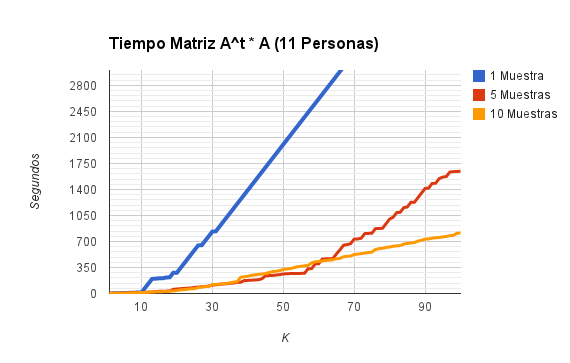
\includegraphics[width=1\textwidth]{img/image1.png}
     \caption{Tiempos Matrix $A^tA$ con 11 personas variando K}
     \label{fig:figura1}
\end{figure}

\begin{figure}[H]
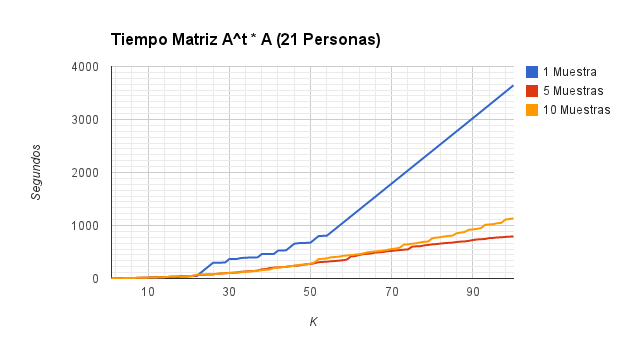
\includegraphics[width=1\textwidth]{img/image2.png}
     \caption{Tiempos Matrix $A^tA$ con 21 personas variando K}
     \label{fig:figura1}
\end{figure}

\begin{figure}[H]
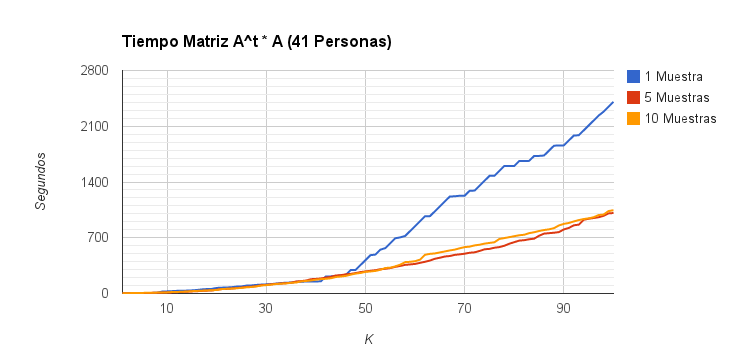
\includegraphics[width=1\textwidth]{img/image3.png}
     \caption{Tiempos Matrix $A^tA$ con 41 personas variando K}
     \label{fig:figura1}
\end{figure}


\textbf{Mediciones de Ttodos }

\begin{figure}[H]
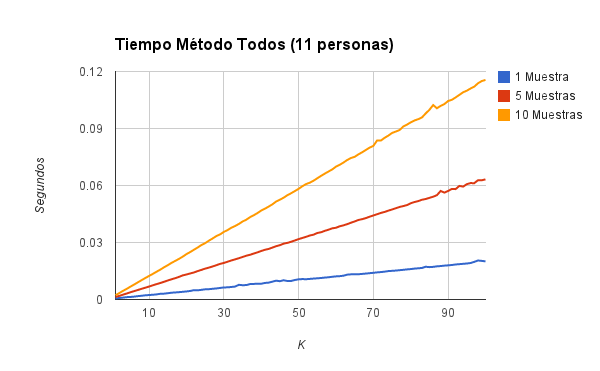
\includegraphics[width=1\textwidth]{img/image4.png}
     \caption{Tiempos Todos \textcolor{red}{??} Matrix $A^tA$ con 11 personas variando K}
     \label{fig:figura1}
\end{figure}

\begin{figure}[H]
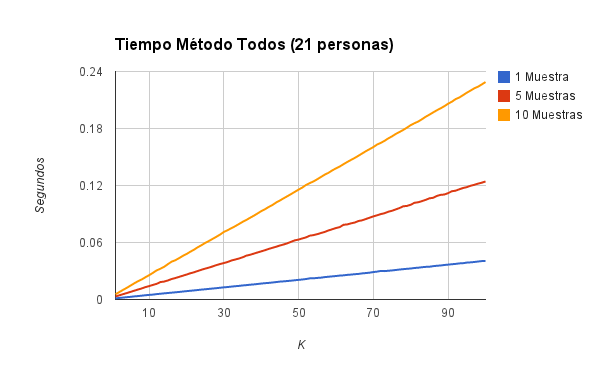
\includegraphics[width=1\textwidth]{img/image5.png}
     \caption{Tiempos Todos \textcolor{red}{??} Matrix $A^tA$ con 21 personas variando K}
     \label{fig:figura1}
\end{figure}

\begin{figure}[H]
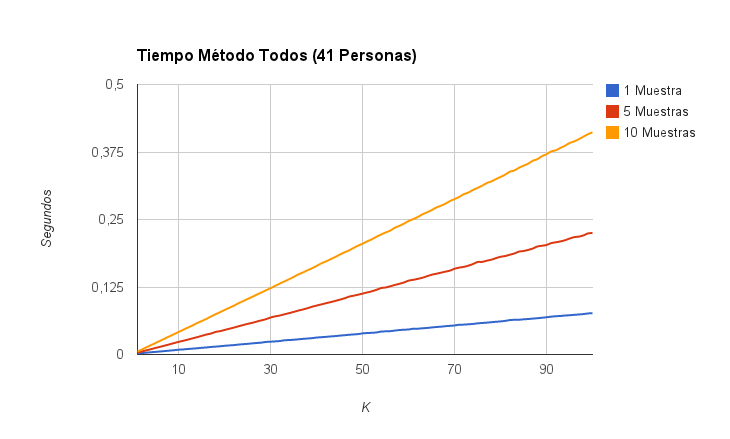
\includegraphics[width=1\textwidth]{img/image6.png}
     \caption{Tiempos Todos \textcolor{red}{??} Matrix $A^tA$ con 41 personas variando K}
     \label{fig:figura1}
\end{figure}


\textbf{Mediciones de Tcentro }

\begin{figure}[H]
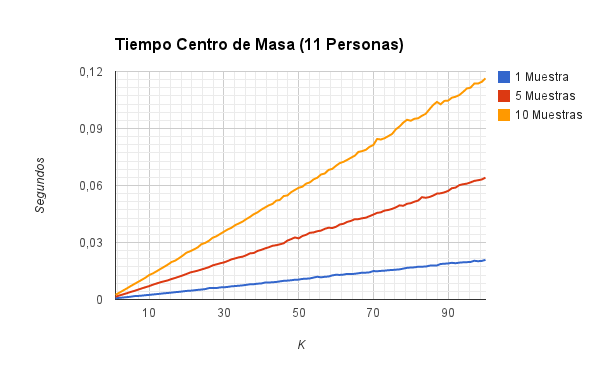
\includegraphics[width=1\textwidth]{img/image7.png}
     \caption{Tiempos Centro \textcolor{red}{??} Matrix $A^tA$ con 11 personas variando K}
     \label{fig:figura1}
\end{figure}

\begin{figure}[H]
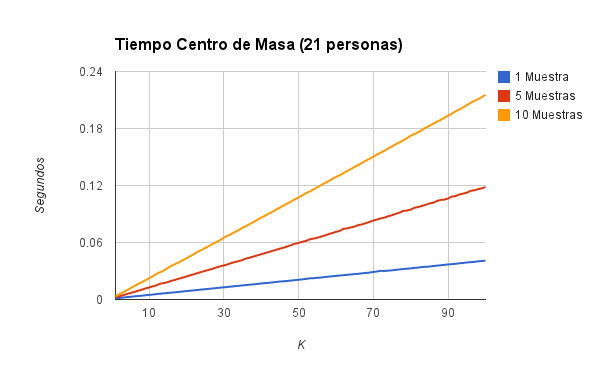
\includegraphics[width=1\textwidth]{img/image8.png}
     \caption{Tiempos Centro \textcolor{red}{??} Matrix $A^tA$ con 21 personas variando K}
     \label{fig:figura1}
\end{figure}

\begin{figure}[H]
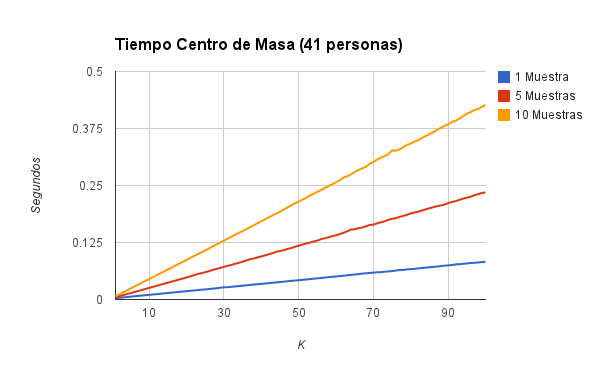
\includegraphics[width=1\textwidth]{img/image9.png}
     \caption{Tiempos Centro \textcolor{red}{??} Matrix $A^tA$ con 41 personas variando K}
     \label{fig:figura1}
\end{figure}



\textbf{Mediciones de HitsTodos }

\begin{figure}[H]
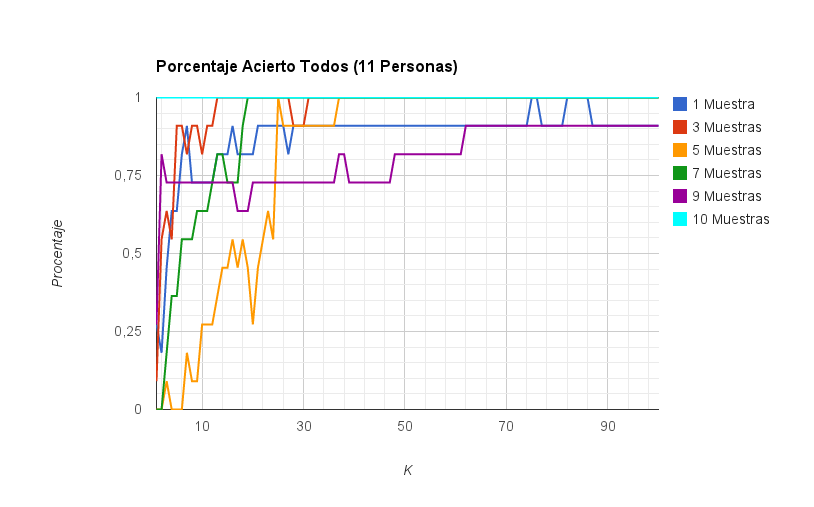
\includegraphics[width=1\textwidth]{img/image10.png}
     \caption{Tiempos HitTodos \textcolor{red}{??} Matrix $A^tA$ con 11 personas variando K}
     \label{fig:figura1}
\end{figure}

\begin{figure}[H]
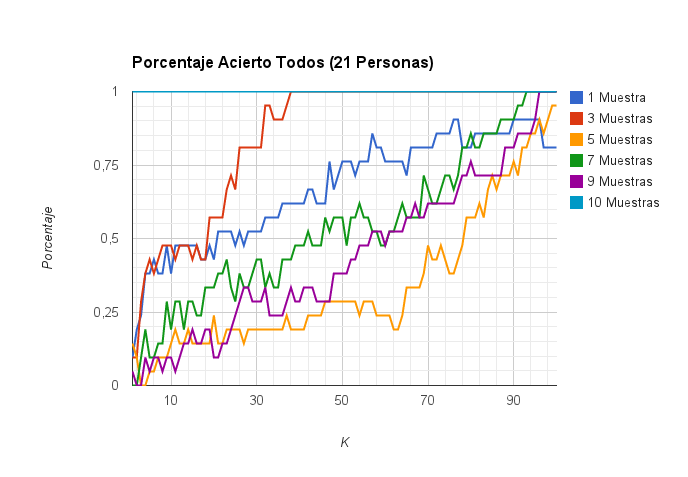
\includegraphics[width=1\textwidth]{img/image11.png}
     \caption{Tiempos HitTodos \textcolor{red}{??} Matrix $A^tA$ con 21 personas variando K}
     \label{fig:figura1}
\end{figure}

\begin{figure}[H]
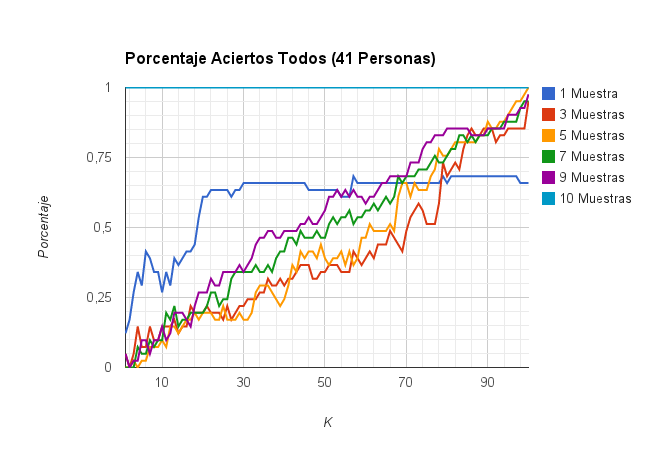
\includegraphics[width=1\textwidth]{img/image12.png}
     \caption{Tiempos HitTodos \textcolor{red}{??} Matrix $A^tA$ con 41 personas variando K}
     \label{fig:figura1}
\end{figure}





\textbf{Mediciones de HitsCentro }

\begin{figure}[H]
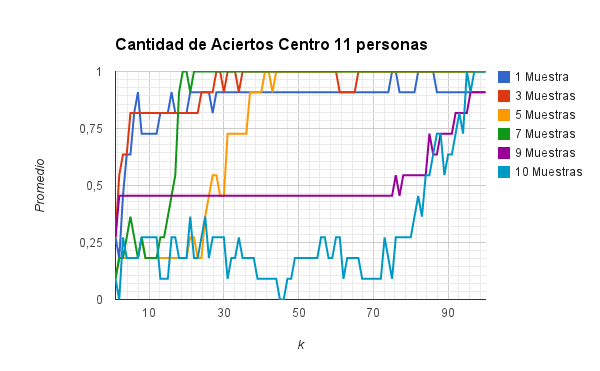
\includegraphics[width=1\textwidth]{img/image13.png}
     \caption{Tiempos HitsCentro \textcolor{red}{??} Matrix $A^tA$ con 11 personas variando K}
     \label{fig:figura1}
\end{figure}

\begin{figure}[H]
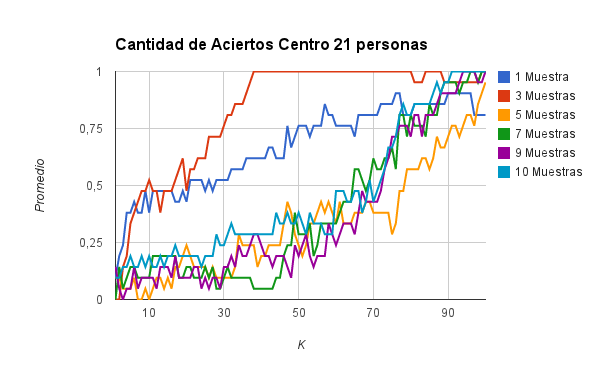
\includegraphics[width=1\textwidth]{img/image14.png}
     \caption{Tiempos HitsCentro \textcolor{red}{??} Matrix $A^tA$ con 21 personas variando K}
     \label{fig:figura1}
\end{figure}

\begin{figure}[H]
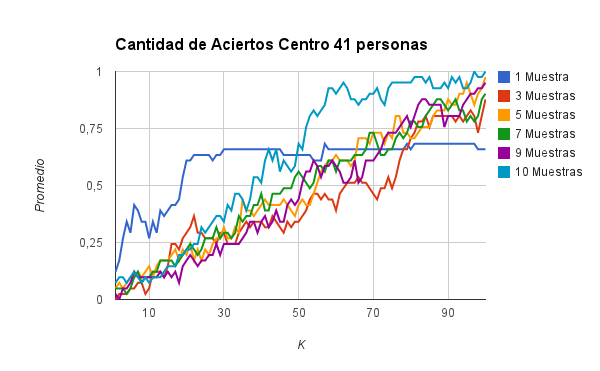
\includegraphics[width=1\textwidth]{img/image15.png}
     \caption{Tiempos HitsCentro \textcolor{red}{??} Matrix $A^tA$ con 41 personas variando K}
     \label{fig:figura1}
\end{figure}

\textbf{Conclusiones:}

\textcolor{red}{EXPLICAR}


\subsubsection{Metodo 1: Utilizando $AA^t$}

\textbf{Mediciones de TK }

\begin{figure}[H]
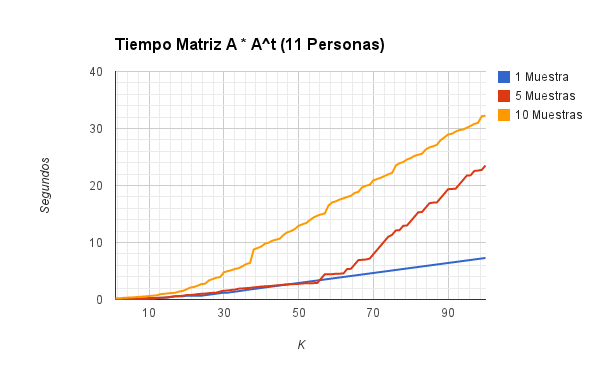
\includegraphics[width=1\textwidth]{img/imagea.png}
     \caption{Tiempos Matrix $A^tA$ con 11 personas variando K}
     \label{fig:figura1}
\end{figure}

\begin{figure}[H]
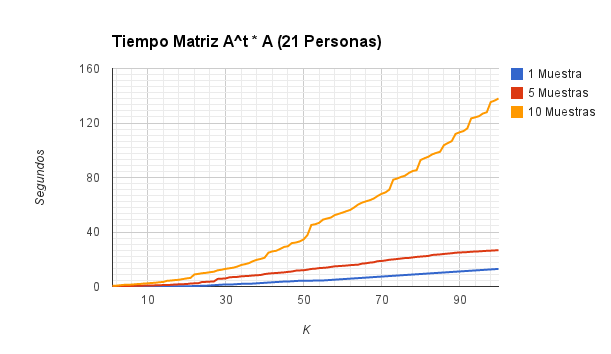
\includegraphics[width=1\textwidth]{img/imageb.png}
     \caption{Tiempos Matrix $A^tA$ con 21 personas variando K}
     \label{fig:figura1}
\end{figure}

\begin{figure}[H]
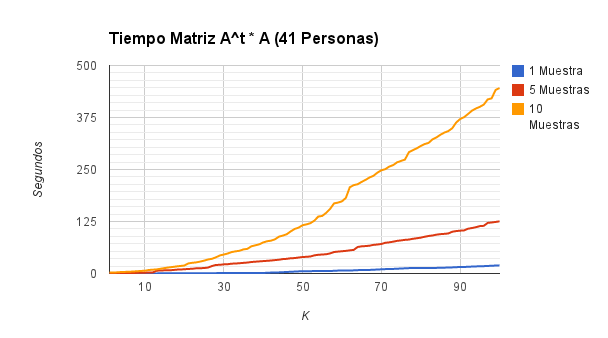
\includegraphics[width=1\textwidth]{img/imagec.png}
     \caption{Tiempos Matrix $A^tA$ con 41 personas variando K}
     \label{fig:figura1}
\end{figure}


\textbf{Mediciones de Ttodos }

\begin{figure}[H]
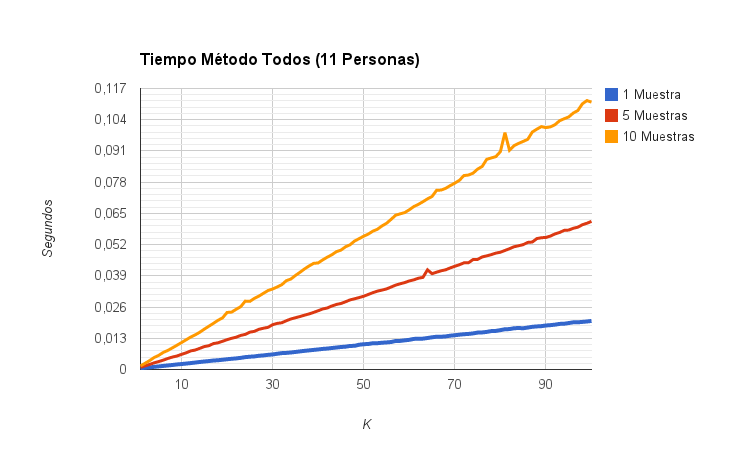
\includegraphics[width=1\textwidth]{img/imaged.png}
     \caption{Tiempos Todos \textcolor{red}{??} Matrix $A^tA$ con 11 personas variando K}
     \label{fig:figura1}
\end{figure}

\begin{figure}[H]
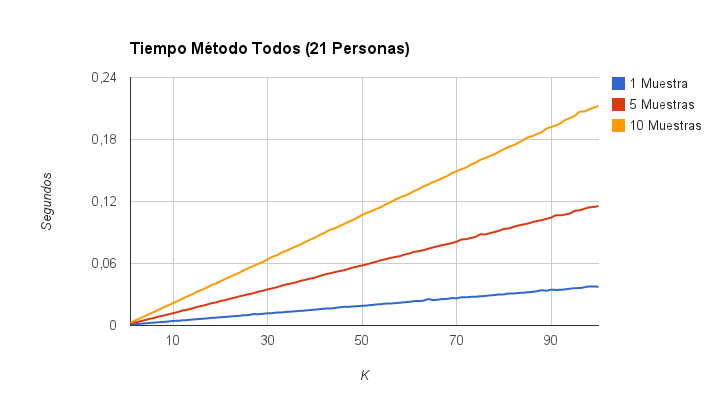
\includegraphics[width=1\textwidth]{img/imagee.png}
     \caption{Tiempos Todos \textcolor{red}{??} Matrix $A^tA$ con 21 personas variando K}
     \label{fig:figura1}
\end{figure}

\begin{figure}[H]
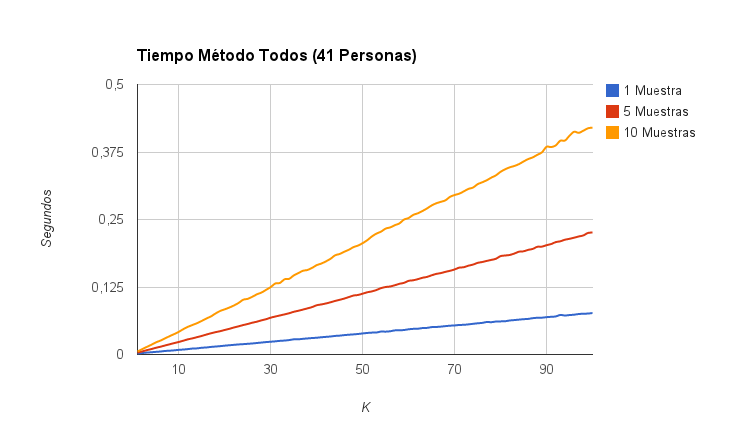
\includegraphics[width=1\textwidth]{img/imagef.png}
     \caption{Tiempos Todos \textcolor{red}{??} Matrix $A^tA$ con 41 personas variando K}
     \label{fig:figura1}
\end{figure}

\textbf{Mediciones de Tcentro }

\begin{figure}[H]
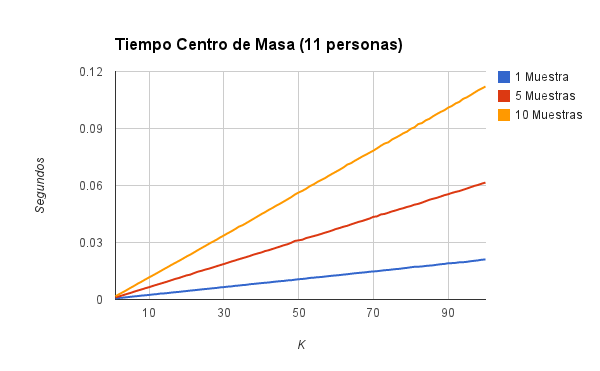
\includegraphics[width=1\textwidth]{img/imageg.png}
     \caption{Tiempos Centro \textcolor{red}{??} Matrix $A^tA$ con 11 personas variando K}
     \label{fig:figura1}
\end{figure}

\begin{figure}[H]
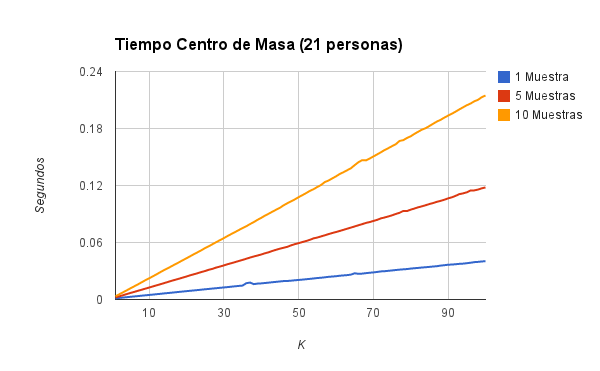
\includegraphics[width=1\textwidth]{img/imageh.png}
     \caption{Tiempos Centro \textcolor{red}{??} Matrix $A^tA$ con 21 personas variando K}
     \label{fig:figura1}
\end{figure}

\begin{figure}[H]
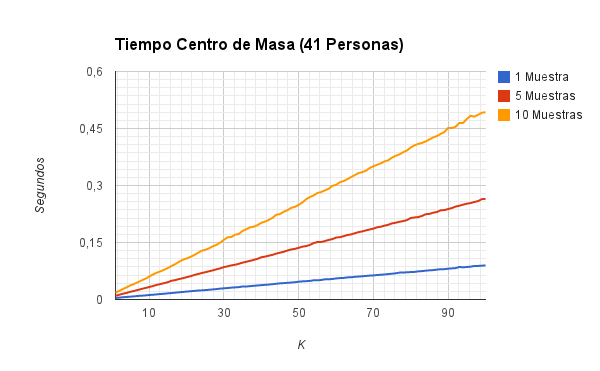
\includegraphics[width=1\textwidth]{img/imagei.png}
     \caption{Tiempos Centro \textcolor{red}{??} Matrix $A^tA$ con 41 personas variando K}
     \label{fig:figura1}
\end{figure}


\textbf{Mediciones de HitsTodos}

\begin{figure}[H]
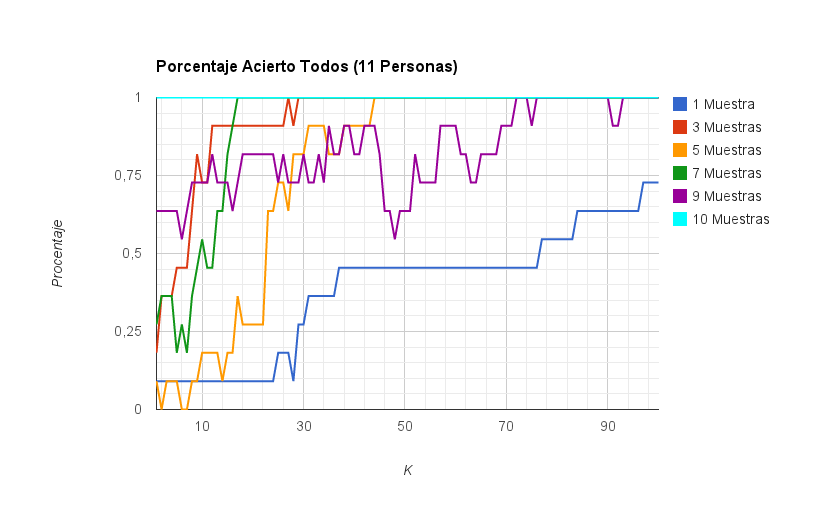
\includegraphics[width=1\textwidth]{img/imagej.png}
     \caption{Tiempos HitTodos \textcolor{red}{??} Matrix $A^tA$ con 11 personas variando K}
     \label{fig:figura1}
\end{figure}

\begin{figure}[H]
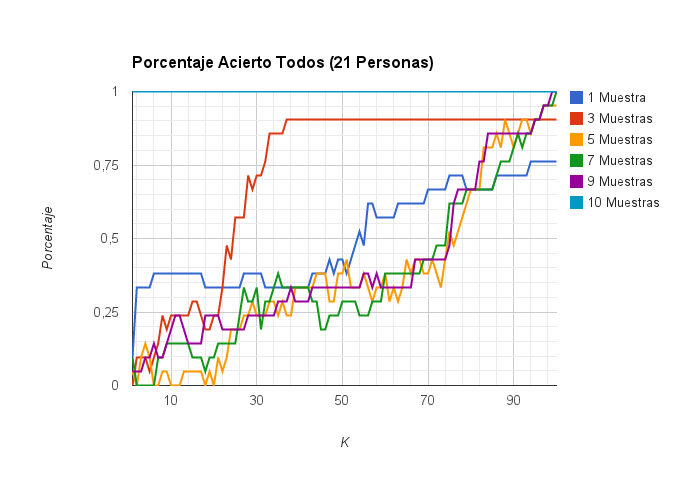
\includegraphics[width=1\textwidth]{img/imagek.png}
     \caption{Tiempos HitTodos \textcolor{red}{??} Matrix $A^tA$ con 21 personas variando K}
     \label{fig:figura1}
\end{figure}

\begin{figure}[H]
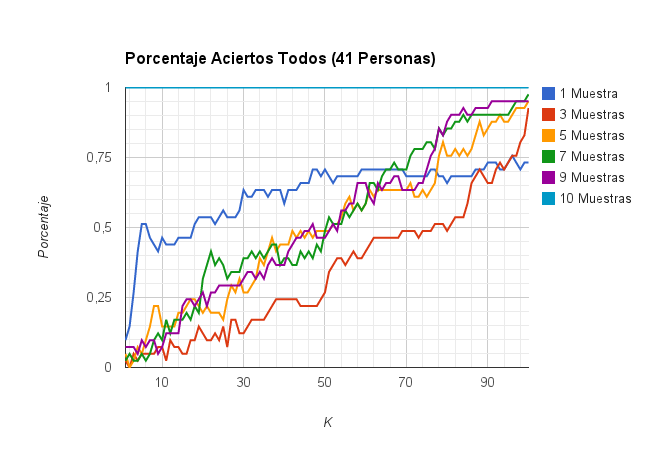
\includegraphics[width=1\textwidth]{img/imagel.png}
     \caption{Tiempos HitTodos \textcolor{red}{??} Matrix $A^tA$ con 41 personas variando K}
     \label{fig:figura1}
\end{figure}

\textbf{Mediciones de HitsCentro}

\begin{figure}[H]
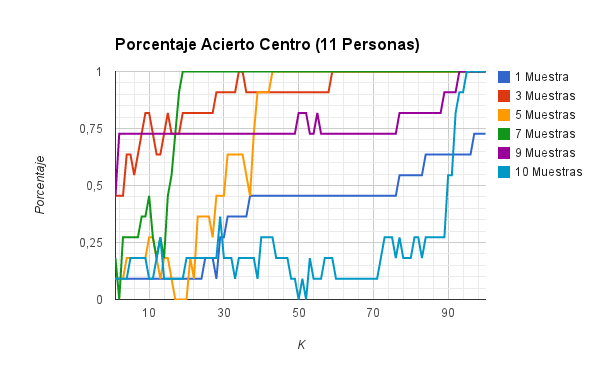
\includegraphics[width=1\textwidth]{img/imagem.png}
     \caption{Tiempos HitsCentro \textcolor{red}{??} Matrix $A^tA$ con 11 personas variando K}
     \label{fig:figura1}
\end{figure}

\begin{figure}[H]
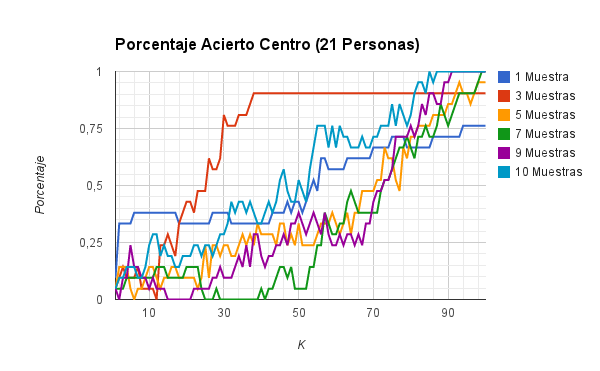
\includegraphics[width=1\textwidth]{img/imagen.png}
     \caption{Tiempos HitsCentro \textcolor{red}{??} Matrix $A^tA$ con 21 personas variando K}
     \label{fig:figura1}
\end{figure}

\begin{figure}[H]
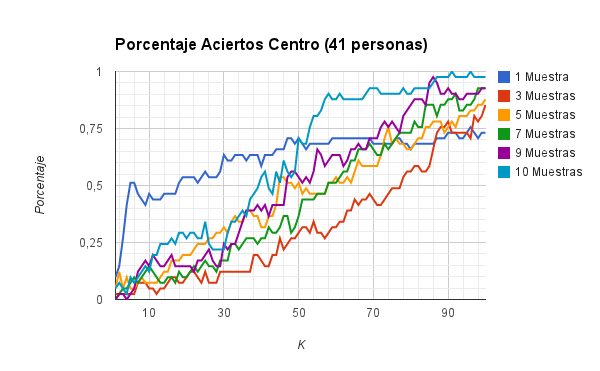
\includegraphics[width=1\textwidth]{img/imager.png}
     \caption{Tiempos HitsCentro \textcolor{red}{??} Matrix $A^tA$ con 41 personas variando K}
     \label{fig:figura1}
\end{figure}

\textbf{Conclusiones:}

\textcolor{red}{EXPLICAR}

\subsection{Experimentacion con Imagenes Full}

\subsubsection{Metodo 0: Utilizando $A^tA$}

\textbf{Mediciones de TK}

\textbf{Mediciones de Ttodos }

\textbf{Mediciones de Tcentro }

\textbf{Mediciones de HitsTodos }

\textbf{Mediciones de HitsCentro}

\textbf{Conclusiones:}

\textcolor{red}{EXPLICAR}

\subsubsection{Metodo 1: Utilizando $AA^t$}

\textbf{Mediciones de TK}

\begin{figure}[H]
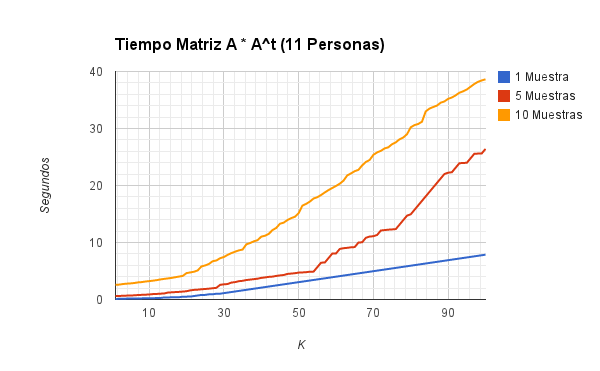
\includegraphics[width=1\textwidth]{img/imagef1.png}
     \caption{Tiempos HitsCentro \textcolor{red}{??} Matrix $A^tA$ con 41 personas variando K}
     \label{fig:figura1}
\end{figure}

\begin{figure}[H]
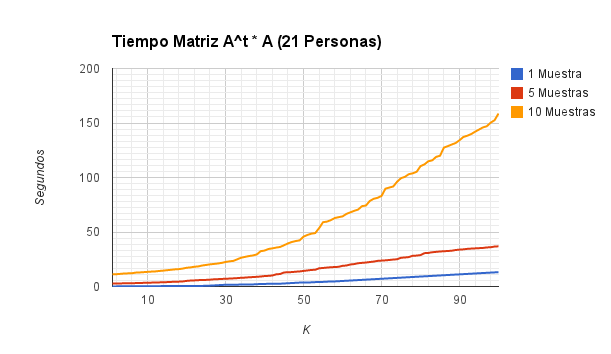
\includegraphics[width=1\textwidth]{img/imagef2.png}
     \caption{Tiempos HitsCentro \textcolor{red}{??} Matrix $A^tA$ con 41 personas variando K}
     \label{fig:figura1}
\end{figure}

\begin{figure}[H]
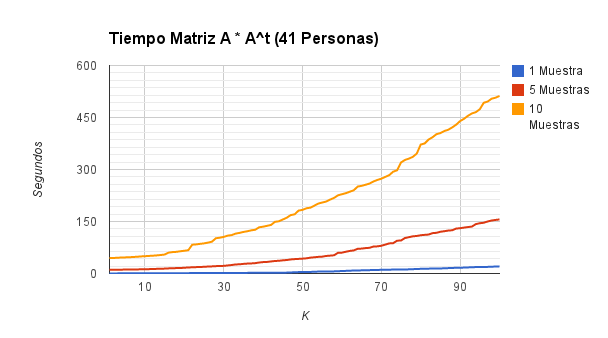
\includegraphics[width=1\textwidth]{img/imagef3.png}
     \caption{Tiempos HitsCentro \textcolor{red}{??} Matrix $A^tA$ con 41 personas variando K}
     \label{fig:figura1}
\end{figure}



\textbf{Mediciones de Ttodos }

\begin{figure}[H]
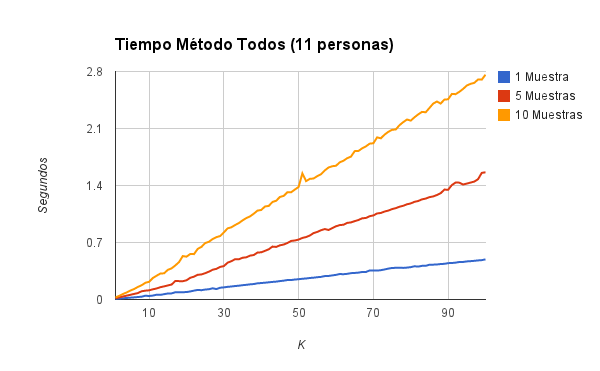
\includegraphics[width=1\textwidth]{img/imagef4.png}
     \caption{Tiempos HitsCentro \textcolor{red}{??} Matrix $A^tA$ con 41 personas variando K}
     \label{fig:figura1}
\end{figure}

\begin{figure}[H]
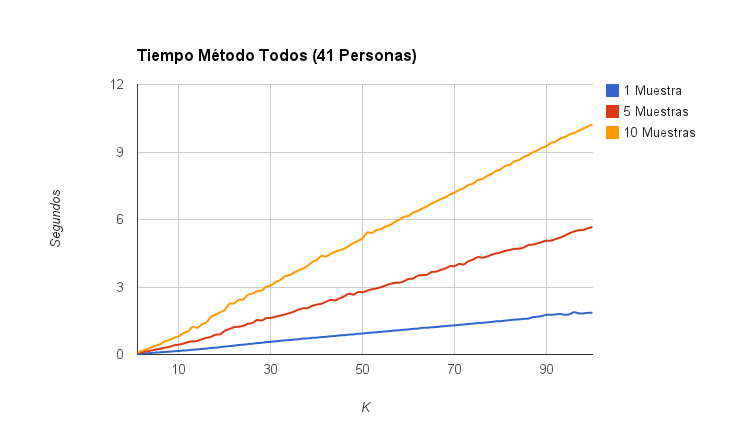
\includegraphics[width=1\textwidth]{img/imagef5.png}
     \caption{Tiempos HitsCentro \textcolor{red}{??} Matrix $A^tA$ con 41 personas variando K}
     \label{fig:figura1}
\end{figure}

\begin{figure}[H]
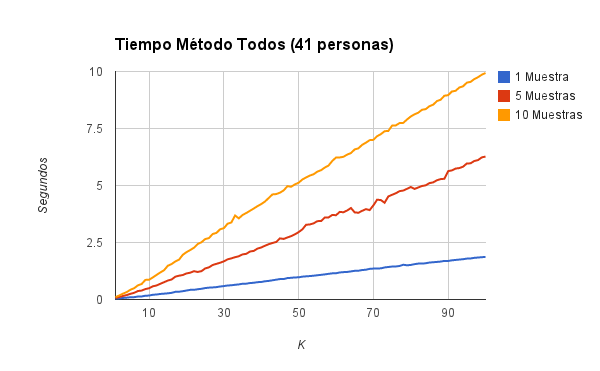
\includegraphics[width=1\textwidth]{img/imagef6.png}
     \caption{Tiempos HitsCentro \textcolor{red}{??} Matrix $A^tA$ con 41 personas variando K}
     \label{fig:figura1}
\end{figure}


\textbf{Mediciones de Tcentro }

\begin{figure}[H]
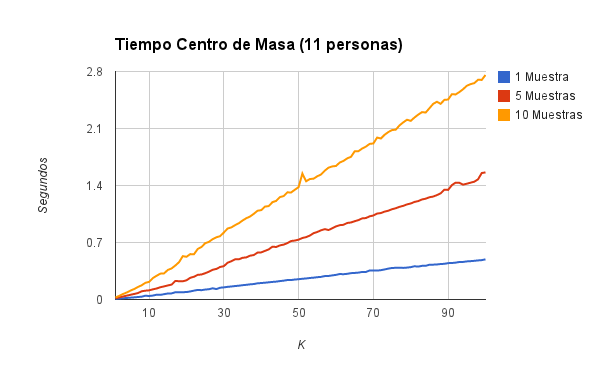
\includegraphics[width=1\textwidth]{img/imagef7.png}
     \caption{Tiempos HitsCentro \textcolor{red}{??} Matrix $A^tA$ con 41 personas variando K}
     \label{fig:figura1}
\end{figure}

\begin{figure}[H]
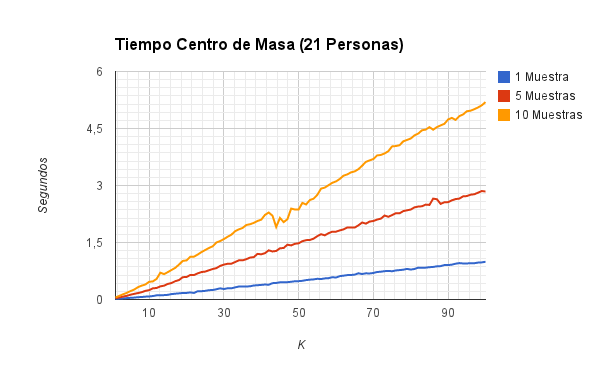
\includegraphics[width=1\textwidth]{img/imagef8.png}
     \caption{Tiempos HitsCentro \textcolor{red}{??} Matrix $A^tA$ con 41 personas variando K}
     \label{fig:figura1}
\end{figure}

\begin{figure}[H]
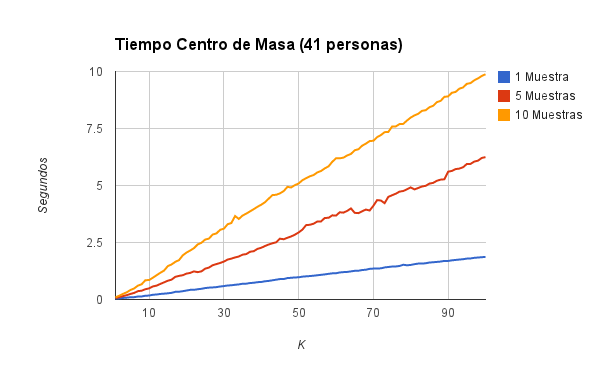
\includegraphics[width=1\textwidth]{img/imagef9.png}
     \caption{Tiempos HitsCentro \textcolor{red}{??} Matrix $A^tA$ con 41 personas variando K}
     \label{fig:figura1}
\end{figure}


\textbf{Mediciones de HitsTodos. }

\begin{figure}[H]
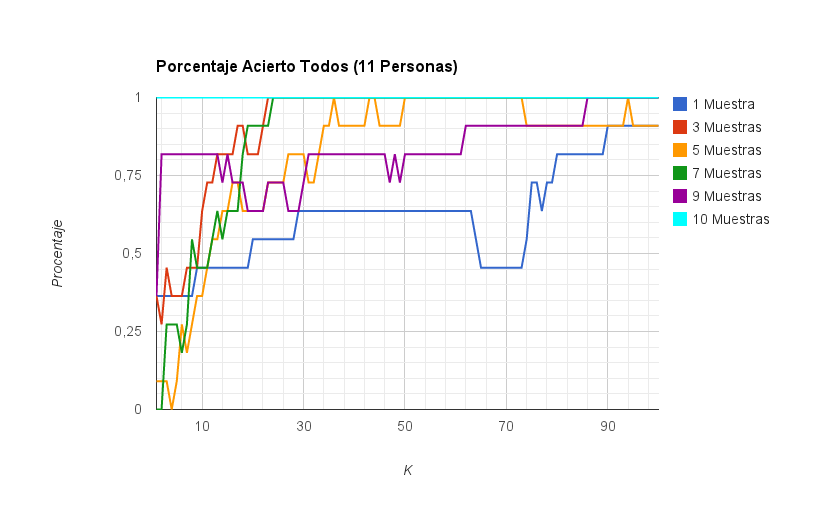
\includegraphics[width=1\textwidth]{img/imagef10.png}
     \caption{Tiempos HitsCentro \textcolor{red}{??} Matrix $A^tA$ con 41 personas variando K}
     \label{fig:figura1}
\end{figure}

\begin{figure}[H]
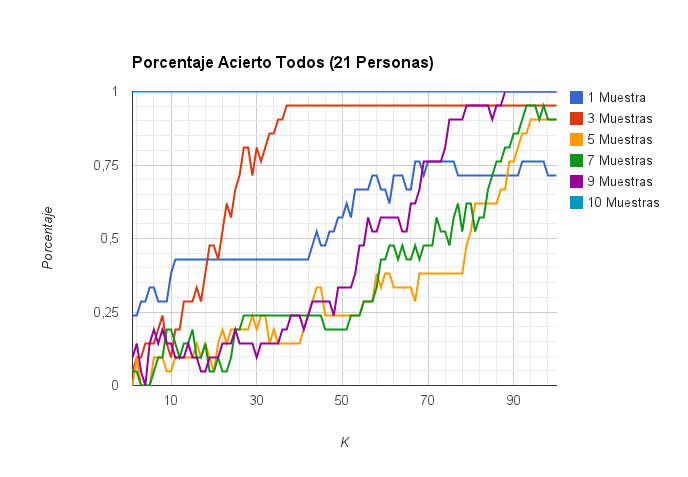
\includegraphics[width=1\textwidth]{img/imagef11.png}
     \caption{Tiempos HitsCentro \textcolor{red}{??} Matrix $A^tA$ con 41 personas variando K}
     \label{fig:figura1}
\end{figure}

\begin{figure}[H]
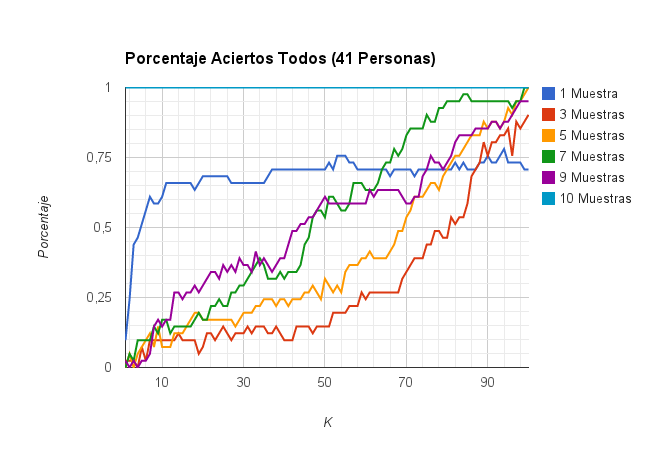
\includegraphics[width=1\textwidth]{img/imagef12.png}
     \caption{Tiempos HitsCentro \textcolor{red}{??} Matrix $A^tA$ con 41 personas variando K}
     \label{fig:figura1}
\end{figure}

\textbf{Mediciones de HitsCentro }

\begin{figure}[H]
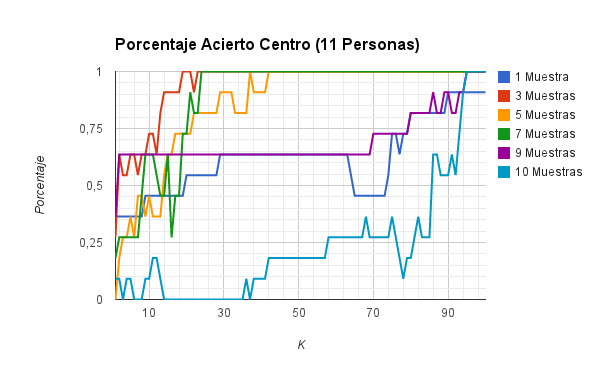
\includegraphics[width=1\textwidth]{img/imagef13.png}
     \caption{Tiempos HitsCentro \textcolor{red}{??} Matrix $A^tA$ con 41 personas variando K}
     \label{fig:figura1}
\end{figure}

\begin{figure}[H]
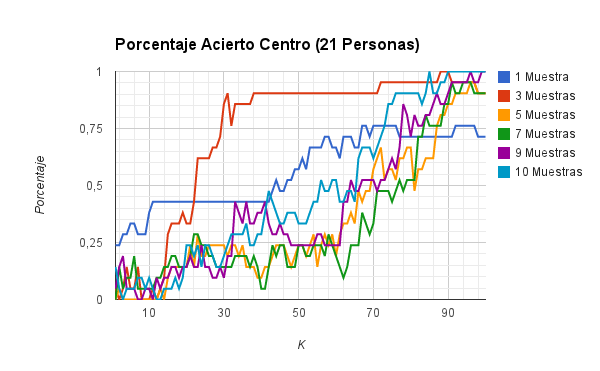
\includegraphics[width=1\textwidth]{img/imagef14.png}
     \caption{Tiempos HitsCentro \textcolor{red}{??} Matrix $A^tA$ con 41 personas variando K}
     \label{fig:figura1}
\end{figure}

\begin{figure}[H]
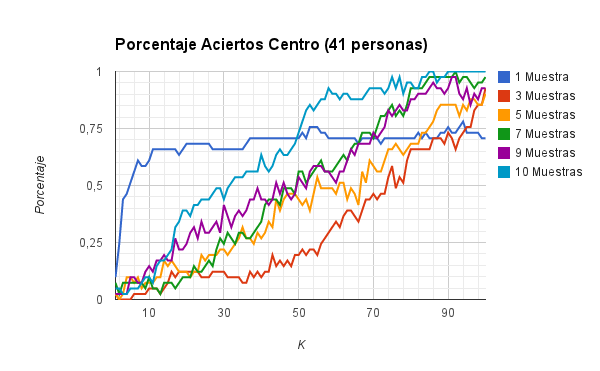
\includegraphics[width=1\textwidth]{img/imagef15.png}
     \caption{Tiempos HitsCentro \textcolor{red}{??} Matrix $A^tA$ con 41 personas variando K}
     \label{fig:figura1}
\end{figure}


\textbf{Conclusiones:}

\textcolor{red}{EXPLICAR}


\newpage

\section{Ap\'endice}
\subsection{Enunciado}


Se pide implementar un programa en \verb+C+ o \verb-C++- que lea desde archivos las im\'agenes de entrenamiento correspondientes a distintas
personas y que, utilizando la descomposici\'on en valores singulares y el n\'umero de componentes principales $k$
mencionado anteriormente, calcule la transformaci\'on caracter\'istica de acuerdo con la descripci\'on anterior. Se debe
proponer e implementar al menos un m\'etodo que, dada una nueva imagen de una cara, determine a que persona de la base
de datos corresponde utilizando la transformaci\'on caracter\'istica.

Con el objetivo de obtener la descomposici\'on en valores singulares, se deber\'a implementar el m\'etodo de la potencia
con deflaci\'on para la estimaci\'on de autovalores/autovectores. En este contexto, la factibilidad de aplicar este
m\'etodo es particularmente sensible al tama\~no de las im\'agenes de la base de datos. Por ejemplo, considerar im\'agenes
en escala de grises de $100 \times 100$ p\'ixeles implicar\'ia trabajar con matrices de tama\~no $10000 \times
10000$. Una alternativa es reducir el tama\~no de las im\'agenes, por ejemplo, mediante un submuestreo. 
Sin embargo, es posible superar esta dificultad en los casos donde el n\'umero de muestras es menor que el
n\'umero de variables. Se pide desarrollar las siguientes sugerencias y fundamentar como utilizarlas en el contexto del
trabajo.

\begin{itemize}
\item Dada una matriz y su descomposici\'on en valores singulares $A = U \Sigma V^t$, encontrar la descomposici\'on en
valores singulares de $A^t$. C\'omo se relacionan los valores singulares de $A$ y $A^t$?
\item Dada la descomposici\'on en valores singulares de $A$, expresar en funci\'on de $U$, $\Sigma$ y $V$ las matrices
$A^t$, $A^tA$ y $AA^t$. Analizar el tama\~no de cada una de ellas y deducir como relacionar las respectivas componentes
principales.
Combinar con el item anterior para el c\'omputo de los componentes principales.
\end{itemize}

En base a este an\'alisis, se pide desarrollar una herramienta alternativa que permita trabajar bajo ciertas condiciones
con im\'agenes de tama\~no mediano/grande.

Junto con este enunciado se provee una base de datos de im\'agenes correspondiente a 41 personas, con 10
im\'agenes por cada una de ellas. Esta base de datos se encuentra disponible en dos resoluciones distintas: $92 \times
112$ y $23 \times 28$ p\'ixeles por cada imagen. La segunda corresponde a un submuestreo de la base original.
En relaci\'on a la experimentaci\'on, se pide como m\'inimo realizar los siguientes experimentos:
\begin{itemize}
\item Analizar para cada una de las variantes qu\'e versi\'on de la base de datos es posible utilizar, en base a
requerimientos de memoria y tiempo de c\'omputo.

\item Para cada una de las variantes propuestas, analizar el impacto en la tasa de efectividad del algoritmo de reconocimiento al
variar la cantidad de componentes principales considerados. Estudiar tambi\'en como impacta la cantidad de im\'agenes
consideradas para cada persona en la etapa de entrenamiento.

\item En caso de considerar m\'as de una posibilidad para determinar a que persona corresponde una nueva cara,
considerar para cada una la mejor configuraci\'on de par\'ametros y compararlas entre ellas.
\end{itemize}

El objetivo final de la experimentaci\'on es proponer una configuraci\'on de par\'armetros/m\'etodos que obtenga
resultados un buen balance entre la tasa de efectividad de reconocimiento de caras, la factibilidad de la propuesta y el
tiempo de c\'omputo requerido.





\subsection{Generador de Tests}

Para generar Tests realizamos un algoritmo en Python en el cual recibimos por parametros el $k$, la cantidad de personas y el metodo a aplicar. Luego variamos la cantidad de personas en un rango de \{1,11,21,31,41\}. Para cada una de estas  variamos la cantidad de imagenes por persona de en el intervalo de 1 a 10 de manera random y comparamos contra una imagen que no sea una muestra (exceptuando el caso en el que cada persona tiene 10 muestras).
El valor de $k$ lo variamos desde adentro del codigo \verb-C++- con el fin de ahorrar calculos ya calculados anteriormente.

\subsection{M\'etodo de compilaci\'on}

\subsubsection{M\'etodo 1}
\begin{framed}
Parados en la carpeta /src del proyecto ejecutar 
\begin{verbatim}
$ make
\end{verbatim}
De esta forma se limpia, compila y ejecutan los test provistos por la c\'atedra.
Para compilar por separado se puede hacer:  \textbf{make data.o}, \textbf{make functions.o}, \textbf{make Matrix.o,} \textbf{make main.o}. O tambien se puede borrar haciendo \textbf{make clean}. Por defecto al ejecutar \textbf{make} el nombre del ejecutable es \textbf{caritas}
\end{framed}

\subsubsection{M\'etodo 2}
\begin{framed}
Parados en la carpeta donde se encuentra el ejecutable (por ejemplo /src/) 
\begin{verbatim}
$ ./ejecutable < PATH TEST IN > <PATH SALIDA> <METODO>
\end{verbatim}
Donde METODO puede ser 
\begin{itemize}
	\item 0: Utiliza para los calculos $A^tA$
	\item 1: Utiliza para los calculos $AA^t$
\end{itemize}
Donde en PATH SALIDA se escriben los autovalores correspondientes.
\end{framed}

\subsection{Script para correr casos}
Dado el tiempo de ejecuci\'on de los casos utilizados para este informe, realizamos un script en python, basadao en el provisto por la c\'atedra, que ejecuta secuencialmente los casos generados previamente y escribiendo el $stdOutput$ de cada caso, en el correspondiente archivo \emph{.console}. //
El script ejecuta solo los casos que no tengan archivos de salida ya generados, por lo que se pueden correr m\'ultiples intancias de este en paralelo.

\subsection{Equipo de pruebas}
Los casos se corrieron sobre un procesador intel i5 de cuatro n\'ucleos sin $hyperthreadying$ y 16GB de memoria ram. Para no afectar las mediciones y optimizar el tiempo, se corrieron tres casos en paralelo continuamente, por lo que se pudo dar el 100\% de un n\'ucleo a todas las pruebas.

\subsection{Referencias bibliogr\'aficas}
\begin{thebibliography}{9}

\bibitem{burden}
  Richard L. Burden and J. Douglas Faires
  \emph{Numerical Analysis}.
  2005.
\end{thebibliography}


\end{document}
